\section{Role-Based Access Control Standard} \label{sec:core-rbac}

RBAC provides effective and efficient permissions management for operations, especially when sharing resources within an organization.
Prior to the creation of the NIST RBAC standard, no general agreement on the definition 
of RBAC existed among practitioners or within the research community. 
Without a unified definition of RBAC, software developers described similar concepts and features of RBAC models using different terminology. 
This lack of consistent terminology was shown to slow the implementation of RBAC~\cite{o20102010}.  
Moreover, in cases where organizations were concerned with adopting RBAC,
evaluation and comparison of RBAC technologies developed by different vendors was difficult.
NIST, in collaboration with industry and academics, worked on defining a set of consensus RBAC concepts and terminology and proposed a standard for 
RBAC that addressed these cost and interoperability issues by developing a common definition that can be used across different vendors.

NIST's work can directly benefit organizations by lowering cost of early phase Research and Development, and implementation of RBAC.
Since the RBAC standard was first introduced, a 2010 report by RTI International showed that the the rate of RBAC adoption has rapidly grown over recent years \cite{o20102010}. 
The analysts estimate that by the end of 2010 at least a portion of permission of systems will use RBAC for more than half of users at organizations with more than 500 employees. The analysts estimate that RBAC technology has generated \$6.1 billion in net economic benefits to industry where NIST RBAC standard work saved \$1.1 billion.

The NIST RBAC standard proposed by Ferraiolo et al. \cite{ferraiolo} and later adopted as the official standard for RBAC by the INCITS includes three components of RBAC: core RBAC, hierarchical RBAC, and constrained RBAC. Each component includes a RBAC reference model. RBAC$_{m}$ includes RBAC reference models of these three components. We first describe the core RBAC, associated entities and other terminology encountered across the space of our review. We next describe hierarchical RBAC and constrained RBAC, which are developed by incorporating new features into the core RBAC. 

\subsection{Core RBAC} 

The four entities of the core RBAC reference model are:

\begin{itemize}
\setlength{\itemsep}{0.25pt}
\item a set of \emph{Users}: A user can be a person or an agent.
\item a set of \emph{Roles}: A role is a collection of permissions to perform a specific job function in an organization.
\item a set of \emph{Permissions}: A permission refers to an access mode that can be exercised on an object in the system and a session relates a user to possibly many roles.
\item a set of \emph{Sessions}: In each session, a user can be assigned to some of the roles, only when the corresponding role is enabled for activation for that time.		
\end{itemize}

In RBAC, a user can exercise a permission only if the user is assigned to a role.
In addition to the four basic entities, two functions are defined:
user assignment ($UA$) and permission assignment ($PA$) functions.
$UA$ assignment of users to roles.
$PA$ assignment of permissions to roles.

\begin{figure}[ht]
    \centering
        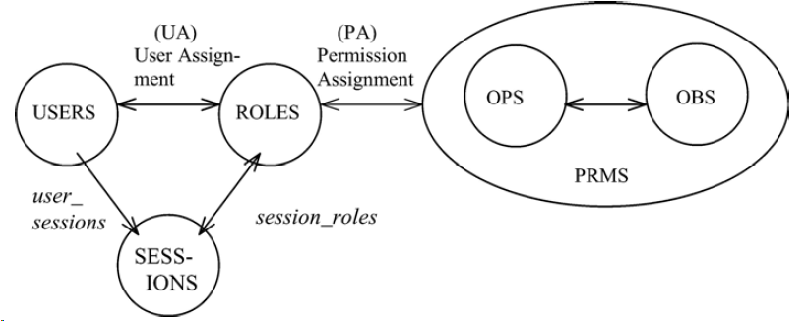
\includegraphics[width=4.0in]{sections/core-model.png}
    \caption{\label{fig:overview}Diagram in Core RBAC reference model\cite{ferraiolokuhn}.}
\end{figure}

Figure~\ref{fig:overview} presents an overview of core RBAC reference model diagram where elements and their relations are described.
Let "USERS", "ROLES", "OBS", "OPS", "PRM", and "SESSIONS" denote users, roles, objects, operations, permissions, and sessions, respectively.
Permissions are associated with possible users' pre-defined operation on an object (e.g., execute a file).
Note that, at user or role activation, a session associated with user or role is established.

\subsection{Hierarchical RBAC} 

The hierarchical RBAC reference model adds role hierarchies ($RH$) feature to the core RBAC reference model.
$RH$ incorporates a structure of roles in an organization using inheritance relationships among attributes such as roles.
The role structure in an organization may use
a role $r_1$, which inherits all permissions of another role $r_2$.
For example, a manager role may inherit all permissions of a employee role.
Role hierarchies help simplify access control policy creation and maintenance by reducing the number of
individual role assignments for a user. Formally, the role inheritance relation is shown as \textit{RH} $\subseteq$ \textit{ROLES} $\times$ \textit{ROLES} describing the many-to-many mapping role inheritance relation. 
General role hierarchies can be extended to use the concept of multiple inheritances where
$r_1$ inherits all permissions from more than one roles.


\subsection{Constrained RBAC}

The constrained RBAC reference model incorporates separation of duty relations to  the core or the hierarchical RBAC reference. Separation of 
duty relations enforces conflict of interest among roles. This model defines two types of separation of duty relations; static and dynamic.

\begin{itemize}
	\item Static Separation of Duty (SSoD): SSoD restricts the conflicting-roles, which can be assigned to a single user statically. Consider that roles $Role_A$ and $Role_B$ are conflicting with each other. On situations
	where multiple roles can be associated with a single user, no permission is given to a user who is assigned to both $Role_A$ and $Role_B$ statically. SSoD is known to be too rigid for practical use in cases where a user should have permissions when a user is assigned to both $Role_A$ and $Role_B$.
	\item Dynamic Separation of Duty (DSD): Dynamic SoD is known to be
more flexible than SSoD. DSD restricts the conflicting-role assignments dynamically that are associated with a user. Consider that roles $Role_A$ and $Role_B$ are conflicting with each other. For the situations where multiple roles can be associated with a single user, no permission is given to a user who is assigned to both $Role_A$ and $Role_B$ dynamically.	
\end{itemize}
